\documentclass{article}
\usepackage{amsmath}
\usepackage{fullpage}
\usepackage{graphicx}
\usepackage{pgfmath}
\usepackage[aux]{rerunfilecheck}
\usepackage{tikz}

\newcommand{\ds}{\displaystyle}

% Macros for MATH 110 course dates

\newcommand{\commonTheme}{metropolis}
\newcommand{\commonColorTheme}{metropolis}

\newcommand{\commonAuthor}{Edward Doolittle}
\newcommand{\commonInstitute}{Department of Indigenous Knowledge and
  Science \\ First Nations University of Canada}
\newcommand{\commonCourse}{MATH 110 Calculus I}
\newcommand{\commonTerm}{202510}
\newcommand{\commonDate}{January 6, 2025}

% Review Material

% Lab 0
\newcommand{\commonEventNegativeOne}{LabNegativeOne}
\newcommand{\commonDateLabNegativeOne}{Monday, January 6, 2025}
\newcommand{\commonTitleLabNegativeOne}{MATH 110 Lab 0}
\newcommand{\commonSubtitleLabNegativeOne}{No Lab; Course Opens}

% Section 001
\newcommand{\commonEventZeroZeroOne}{ZeroZeroOne}
\newcommand{\commonDateZeroZeroOne}{Tuesday, January 7, 2025}
\newcommand{\commonTitleZeroZeroOne}{MATH 110 Review 0.1}
\newcommand{\commonSubtitleZeroZeroOne}{Review of Algebra}
\newcommand{\commonPSTitleZeroZeroOne}{MATH 110 Review Problem Set 0.1}

% Section 00A
\newcommand{\commonEventZeroZeroA}{ZeroZeroA}
\newcommand{\commonDateZeroZeroA}{Tuesday, January 7, 2025}
\newcommand{\commonTitleZeroZeroA}{MATH 110 Review 0.A}
\newcommand{\commonSubtitleZeroZeroA}{Review of Inequalities and
  Absolute Values}
\newcommand{\commonPSTitleZeroZeroA}{MATH 110 Review Problem Set 0.A}

% Section 00B
\newcommand{\commonEventZeroZeroB}{ZeroZeroB}
\newcommand{\commonDateZeroZeroB}{Tuesday, January 7, 2025}
\newcommand{\commonTitleZeroZeroB}{MATH 110 Review 0.B}
\newcommand{\commonSubtitleZeroZeroB}{Review of Coordinate Geometry
  and Lines}
\newcommand{\commonPSTitleZeroZeroB}{MATH 110 Review Problem Set 0.B}

% Section 00C
\newcommand{\commonEventZeroZeroC}{ZeroZeroC}
\newcommand{\commonDateZeroZeroC}{Thursday, January 9, 2025}
\newcommand{\commonTitleZeroZeroC}{MATH 110 Review 0.C}
\newcommand{\commonSubtitleZeroZeroC}{Review of Graphs of Second
  Degree Equations}
\newcommand{\commonPSTitleZeroZeroC}{MATH 110 Review Problem Set 0.C}

% Section 00D
\newcommand{\commonEventZeroZeroD}{ZeroZeroD}
\newcommand{\commonDateZeroZeroD}{Thursday, January 9, 2025}
\newcommand{\commonTitleZeroZeroD}{MATH 110 Review 0.D}
\newcommand{\commonSubtitleZeroZeroD}{Review of Trigonometry}
\newcommand{\commonPSTitleZeroZeroD}{MATH 110 Review Problem Set 0.D}

% Section 011
\newcommand{\commonEventZeroOneOne}{ZeroOneOne}
\newcommand{\commonDateZeroOneOne}{Thursday, January 9, 2025}
\newcommand{\commonTitleZeroOneOne}{MATH 110 Review 1.1}
\newcommand{\commonSubtitleZeroOneOne}{Review of Functions}
\newcommand{\commonPSTitleZeroOneOne}{MATH 110 Review Problem Set 1.1}


% Main Course

% Lab 1
\newcommand{\commonEventZero}{LabZero}
\newcommand{\commonDateLabZero}{Monday, January 13, 2025}
\newcommand{\commonTitleLabZero}{MATH 110 Lab 1}
\newcommand{\commonSubtitleLabZero}{Quiz 0: STACK, Onboarding}

% Section 1.4
\newcommand{\commonEventOne}{ZeroOneFour}
\newcommand{\commonDateZeroOneFour}{Tuesday, January 14, 2025}
\newcommand{\commonTitleZeroOneFour}{MATH 110 Lecture 1.4}
\newcommand{\commonSubtitleZeroOneFour}{The Tangent and Velocity Problems}
\newcommand{\commonPSTitleZeroOneFour}{MATH 110 Problem Set 1.4}

% Section 1.5
\newcommand{\commonEventTwo}{ZeroOneFive}
\newcommand{\commonDateZeroOneFive}{Thursday, January 16, 2025}
\newcommand{\commonTitleZeroOneFive}{MATH 110 Lecture 1.5}
\newcommand{\commonSubtitleZeroOneFive}{The Limit of a Function}
\newcommand{\commonPSTitleZeroOneFive}{MATH 110 Problem Set 1.5}

% Lab 2
\newcommand{\commonEventThree}{LabOne}
\newcommand{\commonDateLabOne}{Monday, January 20, 2025}
\newcommand{\commonTitleLabOne}{MATH 110 Lab 2}
\newcommand{\commonSubtitleLabOne}{Quiz 1: Review}

% Section 1.6
\newcommand{\commonEventFour}{ZeroOneSix}
\newcommand{\commonDateZeroOneSix}{Tuesday, January 21, 2025}
\newcommand{\commonTitleZeroOneSix}{MATH 110 Lecture 1.6}
\newcommand{\commonSubtitleZeroOneSix}{Calculating Limits Using the Limit Laws}
\newcommand{\commonPSTitleZeroOneSix}{MATH 110 Problem Set 1.6}

% Section 1.7
\newcommand{\commonEventFive}{ZeroOneSeven}
\newcommand{\commonDateZeroOneSeven}{(Not covered)}
\newcommand{\commonTitleZeroOneSeven}{MATH 110 Lecture 1.7}
\newcommand{\commonSubtitleZeroOneSeven}{The Precise Definition of a Limit}
\newcommand{\commonPSTitleZeroOneSeven}{MATH 110 Problem Set 1.7}

% Section 1.8
\newcommand{\commonEventSix}{ZeroOneEight}
\newcommand{\commonDateZeroOneEight}{Thursday, January 23, 2025}
\newcommand{\commonTitleZeroOneEight}{MATH 110 Lecture 1.8}
\newcommand{\commonSubtitleZeroOneEight}{Continuity}
\newcommand{\commonPSTitleZeroOneEight}{MATH 110 Problem Set 1.8}

% Lab 3
\newcommand{\commonEventSeven}{LabTwo}
\newcommand{\commonDateLabTwo}{Monday, January 27, 2025}
\newcommand{\commonTitleLabTwo}{MATH 110 Lab 3}
\newcommand{\commonSubtitleLabTwo}{Quiz 2: Sections 1.4, 1.5}

% Section 2.1
\newcommand{\commonEventEight}{ZeroTwoOne}
\newcommand{\commonDateZeroTwoOne}{Tuesday, January 28, 2025}
\newcommand{\commonTitleZeroTwoOne}{MATH 110 Lecture 2.1}
\newcommand{\commonSubtitleZeroTwoOne}{Derivatives and Rates of Change}
\newcommand{\commonPSTitleZeroTwoOne}{MATH 110 Problem Set 2.1}

% Section 2.2
\newcommand{\commonEventNine}{ZeroTwoTwo}
\newcommand{\commonDateZeroTwoTwo}{Thursday, January 30, 2025}
\newcommand{\commonTitleZeroTwoTwo}{MATH 110 Lecture 2.2}
\newcommand{\commonSubtitleZeroTwoTwo}{The Derivative as a Function}
\newcommand{\commonPSTitleZeroTwoTwo}{MATH 110 Problem Set 2.2}

% Lab 4
\newcommand{\commonEventTen}{LabThree}
\newcommand{\commonDateMTOne}{Monday, February 3, 2025} 
\newcommand{\commonDateLabThree}{Monday, February 3, 2025}
\newcommand{\commonTitleLabThree}{MATH 110 Lab 4}
\newcommand{\commonSubtitleLabThree}{Midterm: Review, Chapter 1}

% Section 2.3
\newcommand{\commonEventEleven}{ZeroTwoThree}
\newcommand{\commonDateZeroTwoThree}{Tuesday, February 4, 2025}
\newcommand{\commonTitleZeroTwoThree}{MATH 110 Lecture 2.3}
\newcommand{\commonSubtitleZeroTwoThree}{Differentiation Formulas}
\newcommand{\commonPSTitleZeroTwoThree}{MATH 110 Problem Set 2.3}

% Section 2.4
\newcommand{\commonEventTwelve}{ZeroTwoFour}
\newcommand{\commonDateZeroTwoFour}{Thursday, February 6, 2025}
\newcommand{\commonTitleZeroTwoFour}{MATH 110 Lecture 2.4}
\newcommand{\commonSubtitleZeroTwoFour}{Derivatives of Trigonometric Functions}
\newcommand{\commonPSTitleZeroTwoFour}{MATH 110 Problem Set 2.4}

% Lab 5
\newcommand{\commonEventThirteen}{LabFour}
\newcommand{\commonDateLabFour}{Monday, February 10, 2025}
\newcommand{\commonTitleLabFour}{MATH 110 Lab 5}
\newcommand{\commonSubtitleLabFour}{Quiz 3: Sections 2.1, 2.2}

% Section 2.5
\newcommand{\commonEventFourteen}{ZeroTwoFive}
\newcommand{\commonDateZeroTwoFive}{Tuesday, February 11, 2025}
\newcommand{\commonTitleZeroTwoFive}{MATH 110 Lecture 2.5}
\newcommand{\commonSubtitleZeroTwoFive}{The Chain Rule}
\newcommand{\commonPSTitleZeroTwoFive}{MATH 110 Problem Set 2.5}

% Section 2.6
\newcommand{\commonEventFifteen}{ZeroTwoSix}
\newcommand{\commonDateZeroTwoSix}{Thursday, February 13, 2025}
\newcommand{\commonTitleZeroTwoSix}{MATH 110 Lecture 2.6}
\newcommand{\commonSubtitleZeroTwoSix}{Implicit Differentiation}
\newcommand{\commonPSTitleZeroTwoSix}{MATH 110 Problem Set 2.6}

% Lab 6
\newcommand{\commonEventSixteen}{LabFive}
\newcommand{\commonDateLabFive}{Monday, February 24, 2025}
\newcommand{\commonTitleLabFive}{MATH 110 Lab 6}
\newcommand{\commonSubtitleLabFive}{Quiz 4: Sections 2.3, 2.4}

% Section 2.7
\newcommand{\commonEventSeventeen}{ZeroTwoSeven}
\newcommand{\commonDateZeroTwoSeven}{Tuesday, February 25, 2025}
\newcommand{\commonTitleZeroTwoSeven}{MATH 110 Lecture 2.7}
\newcommand{\commonSubtitleZeroTwoSeven}{Rates of Change in the
  Natural and Social Sciences}
\newcommand{\commonPSTitleZeroTwoSeven}{MATH 110 Problem Set 2.7}

% Section 2.8
\newcommand{\commonEventEighteen}{ZeroTwoEight}
\newcommand{\commonDateZeroTwoEight}{Thursday, February 27, 2025}
\newcommand{\commonTitleZeroTwoEight}{MATH 110 Lecture 2.8}
\newcommand{\commonSubtitleZeroTwoEight}{Related Rates}
\newcommand{\commonPSTitleZeroTwoEight}{MATH 110 Problem Set 2.8}

% Lab 7
\newcommand{\commonEventNineteen}{LabSix}
\newcommand{\commonDateLabSix}{Monday, March 3, 2025}
\newcommand{\commonTitleLabSix}{MATH 110 Lab 7}
\newcommand{\commonSubtitleLabSix}{Quiz 5: Sections 2.5, 2.6}

% Section 3.1
\newcommand{\commonEventTwenty}{ZeroThreeOne}
\newcommand{\commonDateZeroThreeOne}{Tuesday, March 4, 2025}
\newcommand{\commonTitleZeroThreeOne}{MATH 110 Lecture 3.1}
\newcommand{\commonSubtitleZeroThreeOne}{Maximum and Minimum Values}
\newcommand{\commonPSTitleZeroThreeOne}{MATH 11 Problem Set 3.1}

% Section 3.2
\newcommand{\commonEventTwentyOne}{ZeroThreeTwo}
\newcommand{\commonDateZeroThreeTwo}{Thursday, March 6, 2025}
\newcommand{\commonTitleZeroThreeTwo}{MATH 110 Lecture 3.2}
\newcommand{\commonSubtitleZeroThreeTwo}{The Mean Value Theorem}
\newcommand{\commonPSTitleZeroThreeTwo}{MATH 110 Problem Set 3.2}

% Lab 8
\newcommand{\commonEventTwentyTwo}{LabSeven}
\newcommand{\commonDateMTTwo}{Monday, March 10, 2025}
\newcommand{\commonDateLabSeven}{Monday, March 10, 2025}
\newcommand{\commonTitleLabSeven}{MATH 110 Lab 8}
\newcommand{\commonSubtitleLabSeven}{Midterm: Chapter 2}

% Section 3.3
\newcommand{\commonEventTwentyThree}{ZeroThreeThree}
\newcommand{\commonDateZeroThreeThree}{Tuesday, March 11, 2025}
\newcommand{\commonTitleZeroThreeThree}{MATH 110 Lecture 3.3}
\newcommand{\commonSubtitleZeroThreeThree}{How Derivatives Affect the
  Shape of a Graph}
\newcommand{\commonPSTitleZeroThreeThree}{MATH 110 Problem Set 3.3}

% Section 3.4
\newcommand{\commonEventTwentyFour}{ZeroThreeFour}
\newcommand{\commonDateZeroThreeFour}{Thursday, March 13, 2025}
\newcommand{\commonTitleZeroThreeFour}{MATH 110 Lecture 3.4}
\newcommand{\commonSubtitleZeroThreeFour}{Limits at Infinity;
  Horizontal Asymptotes}
\newcommand{\commonPSTitleZeroThreeFour}{MATH 110 Problem Set 3.4}

% Lab 9
\newcommand{\commonEventTwentyFive}{LabEight}
\newcommand{\commonDateLabEight}{Monday, March 17, 2025}
\newcommand{\commonTitleLabEight}{MATH 110 Lab 9}
\newcommand{\commonSubtitleLabEight}{Quiz 6: Sections 3.1, 3.2}

% Section 3.5
\newcommand{\commonEventTwentySix}{ZeroThreeFive}
\newcommand{\commonDateZeroThreeFive}{Tuesday, March 18, 2025}
\newcommand{\commonTitleZeroThreeFive}{MATH 110 Lecture 3.5}
\newcommand{\commonSubtitleZeroThreeFive}{Summary of Curve Sketching}
\newcommand{\commonPSTitleZeroThreeFive}{MATH 110 Problem Set 3.5}

% Section 3.7
\newcommand{\commonEventTwentySeven}{ZeroThreeSeven}
\newcommand{\commonDateZeroThreeSeven}{Thursday, March 20, 2025}
\newcommand{\commonTitleZeroThreeSeven}{MATH 110 Lecture 3.7}
\newcommand{\commonSubtitleZeroThreeSeven}{Optimization Problems}
\newcommand{\commonPSTitleZeroThreeSeven}{MATH 110 Problem Set 3.7}

% Lab 10
\newcommand{\commonEventTwentyEight}{LabNine}
\newcommand{\commonDateLabNine}{Monday, March 24, 2025}
\newcommand{\commonTitleLabNine}{MATH 110 Lab 10}
\newcommand{\commonSubtitleLabNine}{Quiz 7: Sections 3.3, 3.4}

% Section 4.1
\newcommand{\commonEventTwentyNine}{ZeroFourOne}
\newcommand{\commonDateZeroFourOne}{Tuesday, March 25, 2025}
\newcommand{\commonTitleZeroFourOne}{MATH 110 Lecture 4.1}
\newcommand{\commonSubtitleZeroFourOne}{Areas and Distances}
\newcommand{\commonPSTitleZeroFourOne}{MATH 110 Problem Set 4.1}

% Section 4.2
\newcommand{\commonEventThirty}{ZeroFourTwo}
\newcommand{\commonDateZeroFourTwo}{Thursday, March 27, 2025}
\newcommand{\commonTitleZeroFourTwo}{MATH 110 Lecture 4.2}
\newcommand{\commonSubtitleZeroFourTwo}{The Definite Integral}
\newcommand{\commonPSTitleZeroFourTwo}{MATH 110 Problem Set 4.2}

% Lab 11
\newcommand{\commonEventThirtyOne}{LabTen}
\newcommand{\commonDateLabTen}{Monday, March 31, 2025}
\newcommand{\commonTitleLabTen}{MATH 110 Lab 11}
\newcommand{\commonSubtitleLabTen}{Quiz 8: Sections 3.5, 3.7}

% Section 4.3
\newcommand{\commonEventThirtyTwo}{ZeroFourThree}
\newcommand{\commonDateZeroFourThree}{Tuesday, April 1, 2025}
\newcommand{\commonTitleZeroFourThree}{MATH 110 Lecture 4.3}
\newcommand{\commonSubtitleZeroFourThree}{The Fundamental Theorem of Calculus}
\newcommand{\commonPSTitleZeroFourThree}{MATH 110 Problem Set 4.3}

% Section 4.4
\newcommand{\commonEventThirtyThree}{ZeroFourFour}
\newcommand{\commonDateZeroFourFour}{Thursday, April 3, 2025}
\newcommand{\commonTitleZeroFourFour}{MATH 110 Lecture 4.4}
\newcommand{\commonSubtitleZeroFourFour}{Indefinite Integrals and the
  Net Change Theorem}
\newcommand{\commonPSTitleZeroFourFour}{MATH 110 Problem Set 4.4}

% Lab 12
\newcommand{\commonEventThirtyFour}{LabEleven}
\newcommand{\commonDateLabEleven}{Monday, April 7, 2025}
\newcommand{\commonTitleLabEleven}{MATH 110 Lab 12}
\newcommand{\commonSubtitleLabEleven}{Quiz 9: Sections 4.1, 4.2}

% Section 4.5
\newcommand{\commonEventThirtyFive}{ZeroFourFive}
\newcommand{\commonDateZeroFourFive}{Tuesday, April 8, 2025}
\newcommand{\commonTitleZeroFourFive}{MATH 110 Lecture 4.5}
\newcommand{\commonSubtitleZeroFourFive}{The Substitution Rule}
\newcommand{\commonPSTitleZeroFourFive}{MATH 110 Problem Set 4.5}

% Section 5.1
\newcommand{\commonEventThirtySix}{ZeroFiveOne}
\newcommand{\commonDateZeroFiveOne}{Thursday, April 10, 2025}
\newcommand{\commonTitleZeroFiveOne}{MATH 110 Lecture 5.1}
\newcommand{\commonSubtitleZeroFiveOne}{Areas Between Curves}
\newcommand{\commonPSTitleZeroFiveOne}{MATH 110 Problem Set 5.1}

% Lab 13
\newcommand{\commonEventThirtySeven}{LabTwelve}
\newcommand{\commonDateLabTwelve}{Monday, April 14, 2025}
\newcommand{\commonTitleLabTwelve}{MATH 110 Review Lab}
\newcommand{\commonSubtitleLabTwelve}{Bonus Quiz 10: Sections 4.3, 4.4}

% Final Class
\newcommand{\commonEventThirtyEight}{FinalClass}
\newcommand{\commonDateFinalClass}{Tuesday, April 15, 2025}
\newcommand{\commonTitleFinalClass}{MATH 110 Review Class}
\newcommand{\commonSubtitleFinalClass}{Answer Questions, Review for Exam}

% Final Exam
\newcommand{\commonEventThirtyNine}{Final}
\newcommand{\commonDateFinal}{Thursday, April 22, 2025}
\newcommand{\commonTitleFinal}{MATH 110 Final Exam}
\newcommand{\commonSubtitleFinal}{Comprehensive Exam: All Sections}

% Orphaned -- no longer part of the course

% Section 2.9
\newcommand{\commonDateZeroTwoNine}{Not part of the course}
\newcommand{\commonTitleZeroTwoNine}{MATH 110 Lecture 2.9}
\newcommand{\commonSubtitleZeroTwoNine}{Linear Approximations and Differentials}
\newcommand{\commonPSTitleZeroTwoNine}{MATH 110 Problem Set 2.9}


% % Introduction
% \newcommand{\commonEventOneDate}{Wednesday, September 8, 2010}
% \newcommand{\commonEventOneDesc}{Introduction to the Course}
% \newcommand{\commonDateZeroZeroZero}{September 8, 2010}
% \newcommand{\commonTitleZeroZeroZero}{MATH 104 Introduction}
% \newcommand{\commonSubtitleZeroZeroZero}{Outline of the Course}

% % Lecture 1
% \newcommand{\commonEventTwoDate}{Friday, September 10, 2010}
% \newcommand{\commonEventTwoDesc}{Lecture 1: Algebra}
% \newcommand{\commonDateZeroZeroOne}{September 10, 2010}
% \newcommand{\commonTitleZeroZeroOne}{MATH 104 Lecture 1}
% \newcommand{\commonSubtitleZeroZeroOne}{Review of Algebra}
% % associated evaluation ... factor this out?
% \newcommand{\commonPSTitleZeroZeroOne}{MATH 104 Problem Set 1}
% \newcommand{\commonEvalZeroZeroOne}{Quiz 1}
% \newcommand{\commonEvalDateZeroZeroOne}{Wednesday, September 15, 2010}

% % Lecture 2
% \newcommand{\commonEventThreeDate}{Monday, September 13, 2010}
% \newcommand{\commonEventThreeDesc}{Lecture 2: Appendix A}
% \newcommand{\commonDateZeroZeroA}{September 13, 2010}
% \newcommand{\commonTitleZeroZeroA}{MATH 104 Lecture 2}
% \newcommand{\commonSubtitleZeroZeroA}{Appendix A: Numbers, Inequalities, 
%   and Absolute Values}
% % associated evaluation ... factor this out?
% \newcommand{\commonPSTitleZeroZeroA}{MATH 104 Problem Set 2}
% \newcommand{\commonEvalZeroZeroA}{Quiz 2}
% \newcommand{\commonEvalDateZeroZeroA}{Wednesday, September 22, 2010}

% % Review 1
% \newcommand{\commonEventFourDate}{Wednesday, September 15, 2010}
% \newcommand{\commonEventFourDesc}{Review 1: Review Algebra; Quiz 1; Review Appendix A}
% \newcommand{\commonDateRZeroOne}{September 15, 2010}
% \newcommand{\commonTitleRZeroOne}{MATH 104 Review 1}
% \newcommand{\commonSubtitleRZeroOne}{Review of Algebra, Appendix A}

% % Lecture 3
% \newcommand{\commonEventFiveDate}{Friday, September 17, 2010}
% \newcommand{\commonEventFiveDesc}{Lecture 3: Appendix B}
% \newcommand{\commonDateZeroZeroB}{September 17, 2010}
% \newcommand{\commonTitleZeroZeroB}{MATH 104 Lecture 3}
% \newcommand{\commonSubtitleZeroZeroB}{Appendix B: Coordinate Geometry and Lines}
% % associated evaluation ... factor this out?
% \newcommand{\commonPSTitleZeroZeroB}{MATH 104 Problem Set 3}
% \newcommand{\commonEvalZeroZeroB}{Quiz 2}
% \newcommand{\commonEvalDateZeroZeroB}{Wednesday, September 22, 2010}

% % Lecture 4
% \newcommand{\commonEventSixDate}{Monday, Sepbember 20, 2010}
% \newcommand{\commonEventSixDesc}{Lecture 4: Appendix C}
% \newcommand{\commonDateZeroZeroC}{September 20, 2010}
% \newcommand{\commonTitleZeroZeroC}{MATH 104 Lecture 4}
% \newcommand{\commonSubtitleZeroZeroC}{Appendix C: Graphs of Second-Degree Equations}
% % associated evaluation ... factor this out?
% \newcommand{\commonPSTitleZeroZeroC}{MATH 104 Problem Set 4}
% \newcommand{\commonEvalZeroZeroC}{Midterm 0}
% \newcommand{\commonEvalDateZeroZeroC}{Wednesday, September 29, 2010}

% % Review 2
% \newcommand{\commonEventSevenDate}{Wednesday, September 22, 2010}
% \newcommand{\commonEventSevenDesc}{Review 2: Review Appendix B; Quiz 2; Review Appendix C}
% \newcommand{\commonDateRZeroTwo}{September 22, 2010}
% \newcommand{\commonTitleRZeroTwo}{MATH 104 Review 2}
% \newcommand{\commonSubtitleRZeroTwo}{Review of Appendices B and C}

% % Lecture 5
% \newcommand{\commonEventEightDate}{Friday, September 24, 2010}
% \newcommand{\commonEventEightDesc}{Lecture 5: Appendix D}
% \newcommand{\commonDateZeroZeroD}{September 24, 2010}
% \newcommand{\commonTitleZeroZeroD}{MATH 104 Lecture 5}
% \newcommand{\commonSubtitleZeroZeroD}{Appendix D: Trigonometry}
% % associated evaluation ... factor this out?
% \newcommand{\commonPSTitleZeroZeroD}{MATH 104 Problem Set 5}
% \newcommand{\commonEvalZeroZeroD}{Midterm 0}
% \newcommand{\commonEvalDateZeroZeroD}{Wednesday, September 29, 2010}

% % Lecture 6
% \newcommand{\commonEventNineDate}{Monday, September 27, 2010}
% \newcommand{\commonEventNineDesc}{Lecture 6: Section 1.1}
% \newcommand{\commonDateZeroOneOne}{September 27, 2010}
% \newcommand{\commonTitleZeroOneOne}{MATH 104 Lecture 6}
% \newcommand{\commonSubtitleZeroOneOne}{Section 1.1: Four Ways to Represent a Function}
% % associated evaluation ... factor this out?
% \newcommand{\commonPSTitleZeroOneOne}{MATH 104 Problem Set 6}
% \newcommand{\commonEvalZeroOneOne}{Quiz 3}
% \newcommand{\commonEvalDateZeroOneOne}{Wednesday, October 6, 2010}

% % Review 3
% \newcommand{\commonEventTenDate}{Wednesday, September 29, 2010}
% \newcommand{\commonEventTenDesc}{Review 3: Review Appendix D; 
%   Self-Assessment Midterm 0}
% \newcommand{\commonDateRZeroThree}{September 29, 2010}
% \newcommand{\commonTitleRZeroThree}{MATH 104 Review 3}
% \newcommand{\commonSubtitleRZeroThree}{Review of Appendix D}

% % Lecture 7
% \newcommand{\commonEventElevenDate}{Friday, October 1, 2010}
% \newcommand{\commonEventElevenDesc}{Lecture 7: Section 1.2}
% \newcommand{\commonDateZeroOneTwo}{October 1, 2010}
% \newcommand{\commonTitleZeroOneTwo}{MATH 104 Lecture 7}
% \newcommand{\commonSubtitleZeroOneTwo}{Section 1.2: Mathematical Models: A Catalog of Essential Functions}
% % associated evaluation ... factor this out?
% \newcommand{\commonPSTitleZeroOneTwo}{MATH 104 Problem Set 7}
% \newcommand{\commonEvalZeroOneTwo}{Quiz 3}
% \newcommand{\commonEvalDateZeroOneTwo}{Wednesday, October 6, 2010}

% % Lecture 8
% \newcommand{\commonEventTwelveDate}{Monday, October 4, 2010}
% \newcommand{\commonEventTwelveDesc}{Lecture 8: Section 1.3}
% \newcommand{\commonDateZeroOneThree}{October 4, 2010}
% \newcommand{\commonTitleZeroOneThree}{MATH 104 Lecture 8}
% \newcommand{\commonSubtitleZeroOneThree}{Section 1.3: New Functions from Old Functions}
% % associated evaluation ... factor this out?
% \newcommand{\commonPSTitleZeroOneThree}{MATH 104 Problem Set 8}
% \newcommand{\commonEvalZeroOneThree}{Quiz 4}
% \newcommand{\commonEvalDateZeroOneThree}{Wednesday, October 13, 2010}

% % Review 4
% \newcommand{\commonEventThirteenDate}{Wednesday, October 6, 2010}
% \newcommand{\commonEventThirteenDesc}{Review 4: Review 1.1, 1.2; Quiz 3}
% \newcommand{\commonDateROneOne}{October 6, 2010}
% \newcommand{\commonTitleROneOne}{MATH 104 Review 4}
% \newcommand{\commonSubtitleROneOne}{Reveiw of 1.1, 1.2}

% % Lecture 9
% \newcommand{\commonEventFourteenDate}{Friday, October 8, 2010}
% \newcommand{\commonEventFourteenDesc}{Lecture 9: Section 1.4}
% \newcommand{\commonDateZeroOneFour}{October 8, 2010}
% \newcommand{\commonTitleZeroOneFour}{MATH 104 Lecture 9}
% \newcommand{\commonSubtitleZeroOneFour}{Section 1.4: Graphing Calculators and Computers}
% % associated evaluation ... factor this out?
% \newcommand{\commonPSTitleZeroOneFour}{MATH 104 Problem Set 9}
% \newcommand{\commonEvalZeroOneFour}{Quiz 4}
% \newcommand{\commonEvalDateZeroOneFour}{Wednesday, October 13, 2010}

% % Thanksgiving holiday
% \newcommand{\commonEventFifteenDate}{Monday, October 11, 2010}
% \newcommand{\commonEventFifteenDesc}{No class: Thanksgiving holiday}

% % Review 5
% \newcommand{\commonEventSixteenDate}{Wednesday, October 13, 2010}
% \newcommand{\commonEventSixteenDesc}{Review 5: Review 1.3, 1.4; Quiz 4}
% \newcommand{\commonDateROneTwo}{October 13, 2010}
% \newcommand{\commonTitleROneTwo}{MATH 104 Review 5}
% \newcommand{\commonSubtitleOneRTwo}{Review of 1.3, 1.4}

% % Lecture 10
% \newcommand{\commonEventSeventeenDate}{Friday, October 15, 2010}
% \newcommand{\commonEventSeventeenDesc}{Lecture 10: Section 1.5}
% \newcommand{\commonDateZeroOneFive}{October 15, 2010}
% \newcommand{\commonTitleZeroOneFive}{MATH 104 Lecture 10}
% \newcommand{\commonSubtitleZeroOneFive}{Section 1.5: Exponential Functions}
% % associated evaluation ... factor this out?
% \newcommand{\commonPSTitleZeroOneFive}{MATH 104 Problem Set 10}
% \newcommand{\commonEvalZeroOneFive}{Quiz 5}
% \newcommand{\commonEvalDateZeroOneFive}{Wednesday, October 20, 2010}

% % Lecture 11
% \newcommand{\commonEventEighteenDate}{Monday, October 18, 2010}
% \newcommand{\commonEventEighteenDesc}{Lecture 11: Section 1.6}
% \newcommand{\commonDateZeroOneSix}{October 18, 2010}
% \newcommand{\commonTitleZeroOneSix}{MATH 104 Lecture 11}
% \newcommand{\commonSubtitleZeroOneSix}{Section 1.6: Inverse Functions and Logarithms}
% % associated evaluation ... factor this out?
% \newcommand{\commonPSTitleZeroOneSix}{MATH 104 Problem Set 11}
% \newcommand{\commonEvalZeroOneSix}{Midterm 1}
% \newcommand{\commonEvalDateZeroOneSix}{Wednesday, October 27, 2010}

% % Review 6
% \newcommand{\commonEventNineteenDate}{Wednesday, October 20, 2010}
% \newcommand{\commonEventNineteenDesc}{Review 6: Review 1.5; Quiz 5; Review 1.6}
% \newcommand{\commonDateROneThree}{October 20, 2010}
% \newcommand{\commonDateZeroOneR}{October 20, 2010}
% \newcommand{\commonTitleROneThree}{MATH 104 Review 6}
% \newcommand{\commonSubtitleROneThree}{Review of 1.5, 1.6}
% % associated evaluation ... factor this out?
% \newcommand{\commonPSTitleZeroOneR}{MATH 104 Problem Set R1}
% \newcommand{\commonEvalZeroOneR}{Midterm 1}
% \newcommand{\commonEvalDateZeroOneR}{Wednesday, October 27, 2010}

% % Lecture 12
% \newcommand{\commonEventTwentyDate}{Friday, October 22, 2010}
% \newcommand{\commonEventTwentyDesc}{Lecture 12: Section 2.1}
% \newcommand{\commonDateZeroTwoOne}{October 22, 2010}
% \newcommand{\commonTitleZeroTwoOne}{MATH 104 Lecture 12}
% \newcommand{\commonSubtitleZeroTwoOne}{Section 2.1: The Tangent and Velocity Problems}
% % associated evaluation ... factor this out?
% \newcommand{\commonPSTitleZeroTwoOne}{MATH 104 Problem Set 12}
% \newcommand{\commonEvalZeroTwoOne}{Quiz 6}
% \newcommand{\commonEvalDateZeroTwoOne}{Wednesday, November 3, 2010}

% % Lecture 13
% \newcommand{\commonEventTwentyOneDate}{Monday, October 25, 2010}
% \newcommand{\commonEventTwentyOneDesc}{Lecture 13: Section 2.2(a)}
% \newcommand{\commonDateZeroTwoTwoa}{October 25, 2010}
% \newcommand{\commonTitleZeroTwoTwoa}{MATH 104 Lecture 13}
% \newcommand{\commonSubtitleZeroTwoTwoa}{Section 2.2(a): The Limit of a Function I}
% % associated evaluation ... factor this out?
% \newcommand{\commonPSTitleZeroTwoTwoa}{MATH 104 Problem Set 13}
% \newcommand{\commonEvalZeroTwoTwoa}{Quiz 6}
% \newcommand{\commonEvalDateZeroTwoTwoa}{Wednesday, November 3, 2010}

% % Midterm Test 1
% % October 27, 2010
% \newcommand{\commonEventTwentyTwoDate}{Wednesday, October 27, 2010}
% \newcommand{\commonEventTwentyTwoDesc}{Midterm Test 1: Chapter 1}

% % Lecture 14
% \newcommand{\commonEventTwentyThreeDate}{Friday, October 29, 2010}
% \newcommand{\commonEventTwentyThreeDesc}{Lecture 14: Section 2.2(b)}
% \newcommand{\commonDateZeroTwoTwob}{October 29, 2010}
% \newcommand{\commonTitleZeroTwoTwob}{MATH 104 Lecture 14}
% \newcommand{\commonSubtitleZeroTwoTwob}{Section 2.2(b): The Limit of a Function II}
% % associated evaluation ... factor this out?
% \newcommand{\commonPSTitleZeroTwoTwob}{MATH 104 Problem Set 14}
% \newcommand{\commonEvalZeroTwoTwob}{Quiz 6}
% \newcommand{\commonEvalDateZeroTwoTwob}{Wednesday, November 3, 2010}

% % Lecture 15
% \newcommand{\commonEventTwentyFourDate}{Monday, November 1, 2010}
% \newcommand{\commonEventTwentyFourDesc}{Lecture 15: Section 2.3}
% \newcommand{\commonDateZeroTwoThree}{November 1, 2010}
% \newcommand{\commonTitleZeroTwoThree}{MATH 104 Lecture 15}
% \newcommand{\commonSubtitleZeroTwoThree}{Section 2.3: Calculating Limits Using the Limit Laws}
% % associated evaluation ... factor this out?
% \newcommand{\commonPSTitleZeroTwoThree}{MATH 104 Problem Set 15}
% \newcommand{\commonEvalZeroTwoThree}{Quiz 7}
% \newcommand{\commonEvalDateZeroTwoThree}{Wednesday, November 10, 2010}

% % Review 7
% \newcommand{\commonEventTwentyFiveDate}{Wednesday, November 3, 2010}
% \newcommand{\commonEventTwentyFiveDesc}{Review 7: Review 2.1, 2.2; Quiz 6; Review 2.3}
% \newcommand{\commonDateRTwoOne}{November 3, 2010}
% \newcommand{\commonTitleRTwoOne}{MATH 104 Review 7}
% \newcommand{\commonSubtitleRTwoOne}{Review of 2.1, 2.2, 2.3}

% % Lecture 16
% \newcommand{\commonEventTwentySixDate}{Friday, November 5, 2010}
% \newcommand{\commonEventTwentySixDesc}{Lecture 16: Section 2.5}
% \newcommand{\commonDateZeroTwoFive}{November 5, 2010}
% \newcommand{\commonTitleZeroTwoFive}{MATH 104 Lecture 16}
% \newcommand{\commonSubtitleZeroTwoFive}{Section 2.5: Continuity}
% % associated evaluation ... factor this out?
% \newcommand{\commonPSTitleZeroTwoFive}{MATH 104 Problem Set 16}
% \newcommand{\commonEvalZeroTwoFive}{Quiz 7}
% \newcommand{\commonEvalDateZeroTwoFive}{Wednesday, November 10, 2010}

% % Lecture 17
% \newcommand{\commonEventTwentySevenDate}{Monday, November 8, 2010}
% \newcommand{\commonEventTwentySevenDesc}{Lecture 17: Section 2.6}
% \newcommand{\commonDateZeroTwoSix}{November 8, 2010}
% \newcommand{\commonTitleZeroTwoSix}{MATH 104 Lecture 17}
% \newcommand{\commonSubtitleZeroTwoSix}{Section 2.6: Limits at Infinity: Horizontal Asymptotes}
% % associated evaluation ... factor this out?
% \newcommand{\commonPSTitleZeroTwoSix}{MATH 104 Problem Set 17}
% \newcommand{\commonEvalZeroTwoSix}{Quiz 8}
% \newcommand{\commonEvalDateZeroTwoSix}{Wednesday, November 17, 2010}

% % Review 8
% \newcommand{\commonEventTwentyEightDate}{Wednesday, November 10, 2010}
% \newcommand{\commonEventTwentyEightDesc}{Review 8: Review 2.5; Quiz 7; Review 2.6}
% \newcommand{\commonDateRTwoTwo}{November 10, 2010}
% \newcommand{\commonTitleRTwoTwo}{MATH 104 Review 8}
% \newcommand{\commonSubtitleRTwoTwo}{Review of 2.5, 2.6}

% % Lecture 18
% \newcommand{\commonEventTwentyNineDate}{Friday, November 12, 2010}
% \newcommand{\commonEventTwentyNineDesc}{Lecture 18: Section 2.7}
% \newcommand{\commonDateZeroTwoSeven}{November 12, 2010}
% \newcommand{\commonTitleZeroTwoSeven}{MATH 104 Lecture 18}
% \newcommand{\commonSubtitleZeroTwoSeven}{Section 2.7: Derivatives and Rates of Change}
% % associated evaluation ... factor this out?
% \newcommand{\commonPSTitleZeroTwoSeven}{MATH 104 Problem Set 18}
% \newcommand{\commonEvalZeroTwoSeven}{Quiz 8}
% \newcommand{\commonEvalDateZeroTwoSeven}{Wednesday, November 17, 2010}

% % Lecture 19
% \newcommand{\commonEventThirtyDate}{Monday, November 15, 2010}
% \newcommand{\commonEventThirtyDesc}{Lecture 19: Section 2.8}
% \newcommand{\commonDateZeroTwoEight}{November 15, 2010}
% \newcommand{\commonTitleZeroTwoEight}{MATH 104 Lecture 19}
% \newcommand{\commonSubtitleZeroTwoEight}{Section 2.8: The Derivative as a Function}
% % associated evaluation ... factor this out?
% \newcommand{\commonPSTitleZeroTwoEight}{MATH 104 Problem Set 19}
% \newcommand{\commonEvalZeroTwoEight}{Midterm 2}
% \newcommand{\commonEvalDateZeroTwoEight}{Wednesday, November 24, 2010}

% % Review 9
% % November 17, 2010
% \newcommand{\commonEventThirtyOneDate}{Wednesday, November 17, 2010}
% \newcommand{\commonEventThirtyOneDesc}{Review 9: Review 2.7; Quiz 8; Review 2.8}
% \newcommand{\commonDateRTwoThree}{November 17, 2010}
% \newcommand{\commonTitleRTwoThree}{MATH 104 Review 9}
% \newcommand{\commonSubtitleRTwoThree}{Review of 2.7, 2.8}

% % Lecture 20
% \newcommand{\commonEventThirtyTwoDate}{Friday, November 19, 2010}
% \newcommand{\commonEventThirtyTwoDesc}{Lecture 20: Section 3.1}
% \newcommand{\commonDateZeroThreeOne}{November 19, 2010}
% \newcommand{\commonTitleZeroThreeOne}{MATH 104 Lecture 20}
% \newcommand{\commonSubtitleZeroThreeOne}{Section 3.1: Derivatives of Polynomials and Exponential Functions}
% % associated evaluation ... factor this out?
% \newcommand{\commonPSTitleZeroThreeOne}{MATH 104 Problem Set 20}
% \newcommand{\commonEvalZeroThreeOne}{Quiz 9}
% \newcommand{\commonEvalDateZeroThreeOne}{Wednesday, December 1, 2010}

% % Lecture 21
% \newcommand{\commonEventThirtyThreeDate}{Monday, November 22, 2010}
% \newcommand{\commonEventThirtyThreeDesc}{Lecture 21: Section 3.2}
% \newcommand{\commonDateZeroThreeTwo}{November 22, 2010}
% \newcommand{\commonTitleZeroThreeTwo}{MATH 104 Lecture 21}
% \newcommand{\commonSubtitleZeroThreeTwo}{Section 3.2: The Product and Quotient Rules}
% % associated evaluation ... factor this out?
% \newcommand{\commonPSTitleZeroThreeTwo}{MATH 104 Problem Set 21}
% \newcommand{\commonEvalZeroThreeTwo}{Quiz 9}
% \newcommand{\commonEvalDateZeroThreeTwo}{Wednesday, December 1, 2010}

% % Midterm Test 2
% \newcommand{\commonEventThirtyFourDate}{Wednesday, November 24, 2010}
% \newcommand{\commonEventThirtyFourDesc}{Midterm Test 2: Chapter 2}

% % Lecture 22
% \newcommand{\commonEventThirtyFiveDate}{Friday, November 26, 2010}
% \newcommand{\commonEventThirtyFiveDesc}{Lecture 22: Section 3.3}
% \newcommand{\commonDateZeroThreeThree}{November 26, 2010}
% \newcommand{\commonTitleZeroThreeThree}{MATH 104 Lecture 22}
% \newcommand{\commonSubtitleZeroThreeThree}{Section 3.3: Derivatives of Trigonometric Functions}
% % associated evaluation ... factor this out?
% \newcommand{\commonPSTitleZeroThreeThree}{MATH 104 Problem Set 22}
% \newcommand{\commonEvalZeroThreeThree}{Quiz 9}
% \newcommand{\commonEvalDateZeroThreeThree}{Wednesday, December 1, 2010}

% % Lecture 23
% \newcommand{\commonEventThirtySixDate}{Monday, November 29, 2010}
% \newcommand{\commonEventThirtySixDesc}{Lecture 23: Section 3.4}
% \newcommand{\commonDateZeroThreeFour}{November 29, 2010}
% \newcommand{\commonTitleZeroThreeFour}{MATH 104 Lecture 23}
% \newcommand{\commonSubtitleZeroThreeFour}{Section 3.4: The Chain Rule}
% % associated evaluation ... factor this out?
% \newcommand{\commonPSTitleZeroThreeFour}{MATH 104 Problem Set 23}
% \newcommand{\commonEvalZeroThreeFour}{the final exam}
% \newcommand{\commonEvalDateZeroThreeFour}{Monday, December 13, 2010}

% % Review 10
% \newcommand{\commonEventThirtySevenDate}{Wednesday, December 1, 2010}
% \newcommand{\commonEventThirtySevenDesc}{Review 10: Review 3.1, 3.2, 3.3; Quiz 9}
% \newcommand{\commonDateRThreeTwo}{December 1, 2010}
% \newcommand{\commonTitleRThreeTwo}{MATH 104 Review 10}
% \newcommand{\commonSubtitleRThreeTwo}{Review of 3.1, 3.2, 3.3}

% % Lecture 24
% \newcommand{\commonEventThirtyEightDate}{Friday, December 3, 2010}
% \newcommand{\commonEventThirtyEightDesc}{Lecture 24: Section 3.5}
% \newcommand{\commonDateZeroThreeFive}{December 3, 2010}
% \newcommand{\commonTitleZeroThreeFive}{MATH 104 Lecture 24}
% \newcommand{\commonSubtitleZeroThreeFive}{Section 3.5: Implicit Differentiation}
% % associated evaluation ... factor this out?
% \newcommand{\commonPSTitleZeroThreeFive}{MATH 104 Problem Set 24}
% \newcommand{\commonEvalZeroThreeFive}{the final exam}
% \newcommand{\commonEvalDateZeroThreeFive}{Monday, December 13, 2010}

% % Lecture 25
% \newcommand{\commonEventThirtyNineDate}{Monday, December 6, 2010}
% \newcommand{\commonEventThirtyNineDesc}{Lecture 25: Section 3.6}
% \newcommand{\commonDateZeroThreeSix}{December 6, 2010}
% \newcommand{\commonTitleZeroThreeSix}{MATH 104 Lecture 25}
% \newcommand{\commonSubtitleZeroThreeSix}{Section 3.6: Derivatives of Logarithmic Functions}
% % associated evaluation ... factor this out?
% \newcommand{\commonPSTitleZeroThreeSix}{MATH 104 Problem Set 25}
% \newcommand{\commonEvalZeroThreeSix}{the final exam}
% \newcommand{\commonEvalDateZeroThreeSix}{Monday, December 13, 2010}

% % Review 11
% \newcommand{\commonEventFortyDate}{Wednesday, December 8, 2010}
% \newcommand{\commonEventFortyDesc}{(Bonus) Review 11: Review 3.4, 3.5, 3.6}
% \newcommand{\commonDateRThreeThree}{December 8, 2010}
% \newcommand{\commonTitleRThreeThree}{MATH 104 (Bonus) Review 11}
% \newcommand{\commonSubtitleRThreeThree}{Review of 3.4, 3.5, 3.6}

% % Final Exam
% % December 13, 2010
% \newcommand{\commonEventFinalDate}{Monday, December 13, 2010}
% \newcommand{\commonEventFinalDesc}{MATH 104 Final Exam}

%%% Local variables:
%%% mode: latex
%%% TeX-master: "MATH110-Syllabus.tex"
%%% End:

\title{\commonPSTitleZeroThreeTwo\ Solutions}
\author{\commonAuthor}
\date{\commonDateZeroThreeTwo}

\begin{document}
\maketitle
\begin{enumerate}
\item %3
  \begin{enumerate}
  \item %3a
    The function is a polynomial so it is continuous and differentiable
    everywhere, in particular on the given interval; furthermore we have
    \begin{align*}
      f(0)&=(0)^3-(0)^2-6(0)+2=2\\
      f(3)&=3^3-3^2-6(3)+2=27-9-18+2=2
    \end{align*}
    so $f(0)=f(3)$, and $f$ satisfies all the hypotheses of Rolle's Theorem.
    So we know there is a number $c$ in the interval $(0,3)$ at which
    $f'(c)=0$.  We can find $c$ explicitly in this case by solving
    $f'(x)=3x^2-2x-6=0$ or 
    \begin{equation*}
      x = \frac{2\pm \sqrt{(-2)^2-4(3)(-6)}}{2(3)}
      = \frac{2\pm \sqrt{76}}{6}
      \approx 1.7863, -1.1196
    \end{equation*}
    Only the positive root above is in the interval $[0,3]$, so $c\approx
    1.7863$ is the only number satisfying the conclusion of Rolle's Theorem.
  \item %3b
    By our theorems on the continuity and differentiability of trig
    functions, $f(x)$ is continuous and differentiable everywhere, so it
    certainly is in the given closed interval.  Furthermore,
    \begin{align*}
      \cos(2(\pi/8))  
      &= \cos(\pi/4)=\frac{\sqrt{2}}{2}
      \\
      \cos(2(7\pi/8)) 
      &= \cos(7\pi/4) = \cos(2\pi-(\pi/4))=\cos(\pi/4)=\frac{\sqrt{2}}{2}
    \end{align*}
    so $f(\pi/8)=f(7\pi/8)$.  Therefore $f$ satisfies the hypotheses of 
    Rolle's Theorem.  

    Rolle's Theorem guarantees the existence of a number $c\in[\pi/8,7\pi/8]$
    such that $f'(c)=0$.  In this special case we can find $c$ exactly.  
    Taking the derivative we have
    \begin{equation*}
      f'(x)=-2\sin 2x \implies -2\sin 2c = 0 \implies \sin 2c = 0
    \end{equation*}
    The roots of the sine function are at $k\pi$, $k=0,\pm 1, \pm 2, \ldots$.
    That means that $c$ is among the set of numbers
    $k\pi/2$, $k=0,\pm 1, \pm 2, \ldots$.  We need to figure out which of those
    values of $c$ is in the interval $[\pi/8,7\pi/8]$.  Note that if $k\le 0$,
    then $k\pi/2\le 0<\pi/8$, i.e. $k\pi/2$ is outside (to the left of) the
    given interval.  Furthermore if $k>2$ then $k\pi/2>\pi>7\pi/8$ so $k\pi/2$
    is again outside (to the right of) the given interval.  Therefore $k$ must
    be $1$, and in fact $c=\pi/2$ is inside the interval and satisfies 
    $f'(c)=0$.
  \end{enumerate}
\item %4
  \begin{enumerate}
  \item\label{prob:MVT1} %4a
    The function $f(x)=x^3-x^2-6x+2$ is a polynomial so is continuous and
    differentiable everywhere, and the interval $[0,3]$ is a closed interval,
    so the situation satisfies the hypotheses of the MVT.  The slope of the
    secant line connecting the points $(0,f(0))$ and $(3,f(3))$ is
    \begin{equation*}
      m = \frac{f(3)-f(0)}{3-0} = \frac{27-9-18+2-2}{3}=0
    \end{equation*}
    So to satisfy the conclusion of the MVT, we must find a number $c$ such
    that $f'(c)=0$.  The derivative is
    \begin{equation*}
      f'(x)=3x^2-2x-6
    \end{equation*}
    so $f'(c)=0$ means
    \begin{equation*}
      3c^2-2c-6=0 \implies c=\frac{2\pm \sqrt{4-4(3)(-6)}}{2(3)}
      = \frac{1\pm \sqrt{19}}{3} \approx \mbox{$1.7863$ or $-1.1196$}
    \end{equation*}
    The value $c=-1.1196$ lies outside the interval $[0,3]$ so we throw it away.
    Therefore there is only one number $c$ satisfying the conclusion of the
    MVT, namely $c=(1+\sqrt{19})/3\approx 1.7863$.  
    See Figure~\ref{fig:MVT1}.  Note that in 
    Figure~\ref{fig:MVT1}(a), I have graphed the tangent line at $(c,f(c))$ 
    so you can see that it is parallel to the secant line.
    I have graphed the tangent line to show 
    \begin{figure}[htbp]
      \centering
      $\begin{array}{c@{\hspace{0.5in}}c}
      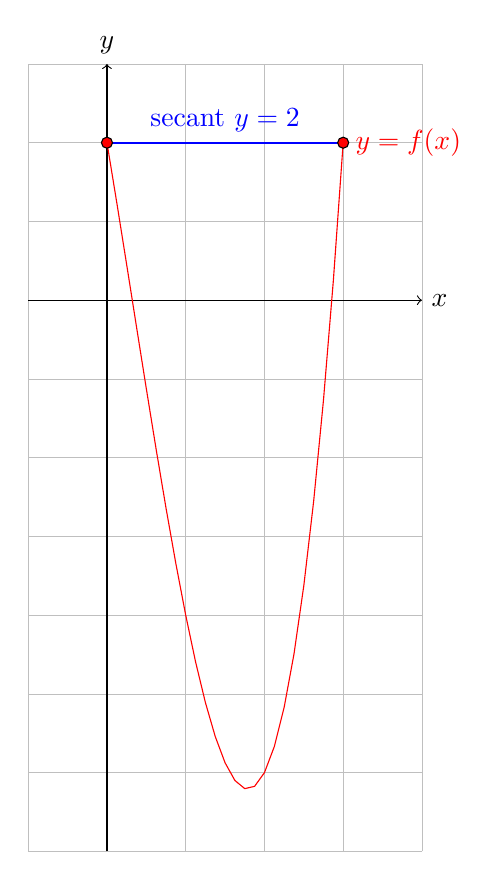
\begin{tikzpicture}
        \draw[very thin,lightgray] (-1,-7) grid (4,3);
        \draw[thin,->] (-1,0)--(4,0) node[right]{$x$};
        \draw[thin,->] (0,-7)--(0,3) node[above]{$y$};
        \draw[domain=0:3,color=red] plot (\x,{(\x)^3-(\x)^2-6*\x+2});
        \draw[thick,color=blue] (0,2)--(3,2) node[midway,above]{secant $y=2$};
        \draw[fill=red] (0,2) circle (2pt) (3,2) circle (2pt) node[right=1pt,color=red]{$y=f(x)$};
      \end{tikzpicture}
      &
      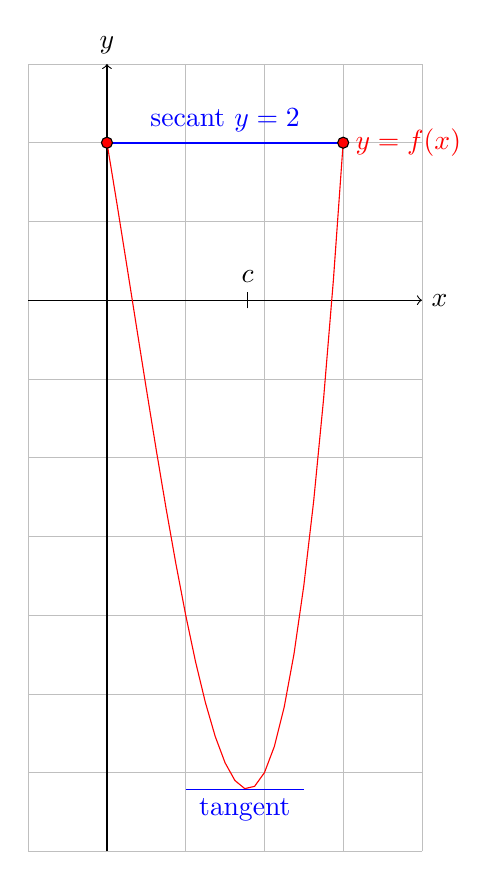
\begin{tikzpicture}
        \draw[very thin,lightgray] (-1,-7) grid (4,3);
        \draw[thin,->] (-1,0)--(4,0) node[right]{$x$};
        \draw[thin] (1.7863,-3pt)--(1.7863,3pt) node[above]{$c$};
        \draw[thin,->] (0,-7)--(0,3) node[above]{$y$};
        \draw[domain=0:3,color=red] plot (\x,{(\x)^3-(\x)^2-6*\x+2});
        \draw[thick,color=blue] (0,2)--(3,2) node[midway,above]{secant $y=2$};
        \draw[fill=red] (0,2) circle (2pt) (3,2) circle (2pt) node[right=1pt,color=red]{$y=f(x)$};
        \draw[color=blue] (1,{(1.7863)^3-(1.7863)^2-6*1.7863+2})--(2.5,{(1.7863)^3-(1.7863)^2-6*1.7863+2}) node[midway,below]{tangent};
      \end{tikzpicture}
      \\
      \mbox{(a) Graph with secant line} 
      & \mbox{(b) Graph with secant and tangent lines}
      \end{array}$
      \caption{Graph of $f(x)=x^3-x^2-6x+2$ for problem~\ref{prob:MVT1}}
      \label{fig:MVT1}
    \end{figure}
  \item\label{prob:MVT2} %4b
    The function $f(x)=x/(x+2)$ is continuous and differentiable
    everywhere except at $x=-2$
    which is outside the given interval $[1,4]$, so $f$ is continuous and 
    differentiable on that interval, so satisfies the conditions of the MVT.
    The slope of the secant line connecting the endpoints $(1,f(1))$ and
    $(4,f(4))$ of the graph is
    \begin{equation*}
      m = \frac{f(4)-f(1)}{4-1} = \frac{\frac{4}{4+2}-\frac{1}{1+2}}{3}
      = \frac{\frac{2}{3}-\frac{1}{3}}{3} = \frac{1}{9}
    \end{equation*}
    To satisfy the conclusion of Rolle's Theorem we need to find a number 
    $c\in[1,4]$ such that $f'(c)=1/9$.  Calculating the derivative,
    \begin{equation*}
      f'(x) = \frac{(x+2)-x}{(x+2)^2} = \frac{2}{(x+2)^2}
    \end{equation*}
    so we have to find $c$ satisfying 
    \begin{equation*}
      f'(c)=\frac{1}{9} \implies \frac{2}{(c+2)^2} = \frac{1}{9}
      \implies (c+2)^2=18 \implies c=-2\pm 3\sqrt{2} \approx \mbox{$2.2426$
      or $-6.2426$}
    \end{equation*}
    Since the negative solution is outside the interval $[1,4]$, we throw it
    away, and obtain just one value $c\approx 2.2426$ which satisfies the
    conclusion of the mean value theorem.  See Figure~\ref{fig:MVT2}.
    \begin{figure}[htbp]
      \centering
      $\begin{array}{c@{\hspace{0.5in}}c}
      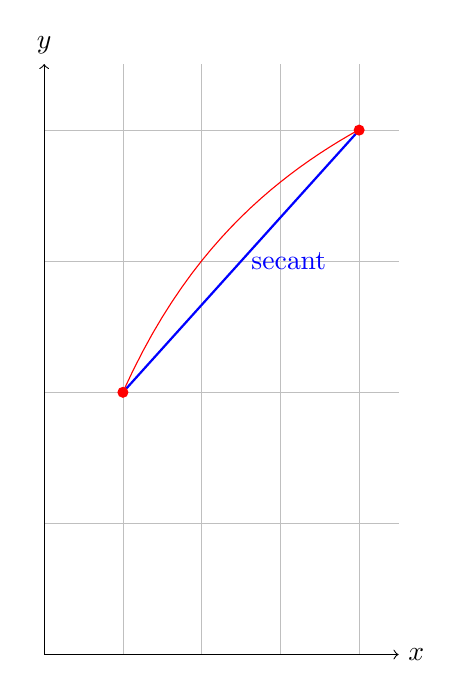
\begin{tikzpicture}[yscale=10]
        \draw[very thin,lightgray,ystep=0.1666] (0,0) grid (4.5,0.75);
        \draw[thin,->] (0,0)--(4.5,0) node[right]{$x$};
        \draw[thin,->] (0,0)--(0,0.75) node[above]{$y$};
        \draw[domain=1:4,color=red] plot (\x,{\x/(\x+2)});
        \draw[thick,color=blue] (1,0.333)--(4,0.666) node[midway,right]{secant};
        \node[shape=circle,fill=red,inner sep=1pt,minimum size=4pt] at (1,0.333){};
        \node[shape=circle,fill=red,inner sep=1pt,minimum size=4pt] at (4,0.666){};
      \end{tikzpicture}
      &
      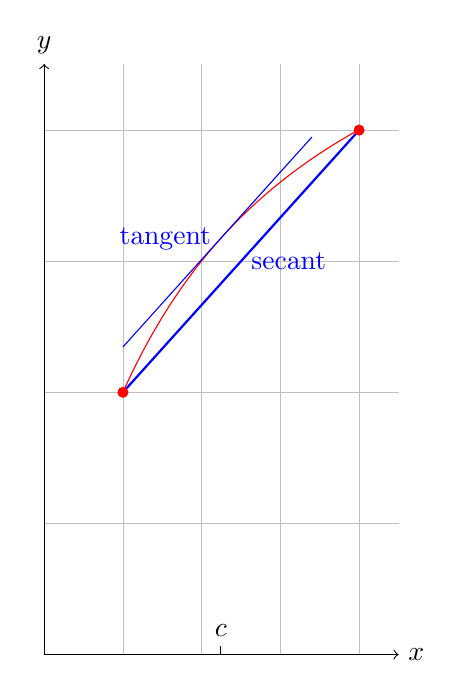
\begin{tikzpicture}[yscale=10]
        \draw[very thin,lightgray,ystep=0.1666] (0,0) grid (4.5,0.75);
        \draw[thin,->] (0,0)--(4.5,0) node[right]{$x$};
        \draw[thin] (2.2426,0)--(2.2426,0.3pt) node[above]{$c$};
        \draw[thin,->] (0,0)--(0,0.75) node[above]{$y$};
        \draw[domain=1:4,color=red] plot (\x,{\x/(\x+2)});
        \draw[thick,color=blue] (1,0.333)--(4,0.666) node[midway,right]{secant};
        \node[shape=circle,fill=red,inner sep=1pt,minimum size=4pt] at (1,0.333){};
        \node[shape=circle,fill=red,inner sep=1pt,minimum size=4pt] at (4,0.666){};
        \draw[domain=1:3.4,color=blue] plot (\x,{1/9*(\x-2.2426)+(2.2426/4.2426)});
        \node[left,color=blue] at (2.2426,{2.2426/4.2426}) {tangent};
      \end{tikzpicture}
      \\
      \mbox{(a) Graph with secant line} 
      & \mbox{(b) Graph with secant and tangent lines}
      \end{array}$
      \caption{Graph of $f(x)=x/(x+2)$ for problem~\ref{prob:MVT2}}
      \label{fig:MVT2}
    \end{figure}
  \end{enumerate}
\item\label{prob:x23} %6
  Note that your calculator may have trouble with $(-1)^{2/3}$.  We have 
  \begin{align*}
    f(-1)&=1-(-1)^{2/3}=1-((-1)^2)^{1/3}=1-(1)^{1/3}=1-1=0 \\
    f(1)&=1-(1)^{2/3}=1-((1)^2)^{1/3}=1-(1)^{1/3}=1-1=0 
  \end{align*}
  so $f(-1)=f(0)$.  Taking the derivative, we have
  \begin{equation*}
    f'(x) = \frac{2}{3} x^{-1/3} = \frac{2}{3\sqrt[3]{x}}
  \end{equation*}
  Note that
  \begin{equation*}
    f'(c)=0 \implies \frac{2}{3\sqrt[3]{c}} = 0
  \end{equation*}
  Multiplying through by $3\sqrt[3]{c}$,
  \begin{equation*}
    \frac{2}{3\sqrt[3]{c}} = 0 \implies 2 = 0
  \end{equation*}
  which is impossible, leading to the conclusion that the equation $f'(c)=0$
  has no solution.  On the other hand, Rolle's Theorem would suggest that
  $f(-1)=f(1)$ implies $f'(c)=0$ for some c in $[-1,1]$, so there is an
  apparent paradox here.

  The solution is that $f(x)$ does not satisfy all the hypotheses of Rolle's
  theorem.  The function is continuous everywhere, but its derivative
  $f'(x)=2/(3\sqrt[3]{x})$ does not exist at $x=0$ (because we would end up
  dividing by $0$).  That single point in $[-1,1]$ where $f'(x)$ does not
  exist is enough to void the application of Rolle's Theorem.  This
  \textit{counterexample} shows that the hypothesis that $f'(x)$ is
  differentiable at every point in the interval $(a,b)$ is required for Rolle's
  Theorem.  See Figure~\ref{fig:x23}.
  \begin{figure}[htbp]
    \centering
    \begin{tikzpicture}[scale=2]
      \draw[very thin,lightgray] (-2,-1) grid (2,2);
      \draw[->] (-2,0)--(2,0) node[right]{$x$};
      \draw[->] (0,-1)--(0,2) node[above]{$y$};
      \draw[color=red,smooth,domain=0.001:1,samples=50] plot (\x,{1-(\x)^(2/3)});
      \draw[color=red,smooth,domain=-1:-0.001,samples=50] plot (\x,{1-(abs(\x))^(2/3)});
      \node[fill=red,shape=circle,inner sep=1pt,minimum size=3pt] at (-1,0) {};
      \node[fill=red,shape=circle,inner sep=1pt,minimum size=3pt] at (1,0) {};
    \end{tikzpicture}
    \caption{Graph of $f(x)=1-x^{2/3}$ for problem~\ref{prob:x23}}
    \label{fig:x23}
  \end{figure}
  Note that $f(x)$ has a cusp at $x=0$ because the one-sided limits of $f'(x)$
  are $+\infty$ on the left and $-\infty$ on the right.
\item\label{prob:x-3-2} %7
  We have
  \begin{align*}
    f(4)      &= (4-3)^{-2} = 1^{-2} = 1 \\
    f(1)      &= (1-3)^{-2} = (-2)^{-2} = \frac{1}{(-2)^2} = \frac{1}{4} \\
    f(4)-f(1) &= \frac{3}{4}
  \end{align*}
  Calculating the derivative,
  \begin{equation*}
    f'(x) = -2(x-3)^{-3} \frac{d}{dx} (x-3) = -2(x-3)^{-3}
  \end{equation*}
  So the MVT would seem to predict that there is a number $c\in(1,4)$ such that
  \begin{equation*}
    f(4)-f(1) = f'(c)(4-1) 
    \implies \frac{3}{4} = -2(c-3)^{-3} (3)
    \implies (c-3)^{-3}=-\frac{1}{8} 
  \end{equation*}
  Taking both sides to the power $-1/3$,
  \begin{equation*}
    \implies c-3=\left(-\frac{1}{8}\right)^{-1/3}=-2
    \implies c=3-2=1
  \end{equation*}
  However, that number $c=1$ is \textit{not} in the open interval $(1,4)$
  because an open interval excludes its end points.  This would seem to 
  violate the MVT, which predicts a number $c$ in the \textit{open} interval
  $(1,4)$ satisfying $f(4)-f(1)=f'(c)(4-1)$.

  Again, the solution is that the hypotheses of the MVT are not satisfied.
  In this case, two hypotheses are not satisfied: $f(x)$ is not continuous
  on the interval $[1,4]$ and $f(x)$ is not differentiable on the interval
  $(1,4)$.  Let's see why.  We rewrite
  \begin{equation*}
    f(x) = (x-3)^{-2} = \frac{1}{(x-3)^2}
  \end{equation*}
  and in that fraction form it is clear that $f(3)$ is undefined at $3\in[1,4]$
  because there is a division by $0$.  Similarly,
  \begin{equation*}
    f'(x) = -2(x-3)^{-3} = -\frac{2}{(x-3)^3}
  \end{equation*}
  is again undefined at $3\in(1,4)$ because there is division by $0$.  The
  moral of this story is that it may be better to rewrite expressions 
  involving negative exponents in terms of positive exponents and fractions
  if we are checking for continuity or differentiability.  See Figure
  \begin{figure}[htbp]
    \centering
    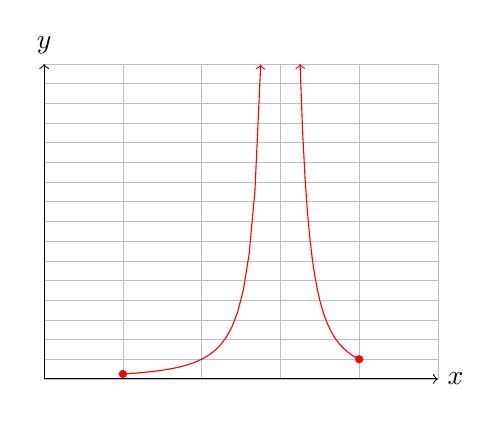
\begin{tikzpicture}[yscale=0.25]
      % note that the inverse function of $f$ is $g(y)=3\pm1/\sqrt{y}$
      % so if we want height to be 4 units we go to 3-1/2, 3+1/2
      % if we want height to be 9 units we go to 3-1/3, 3+1/3
      % if we want height to be 16 units we go to 3-1/4, 3+1/4
      \draw[very thin,lightgray] (0,0) grid (5,16);
      \draw[->] (0,0)--(5,0) node[right]{$x$};
      \draw[->] (0,0)--(0,16) node[above]{$y$};
      \draw[color=red,->,domain=1:2.75] plot (\x,{1/(\x-3)^2});
      \draw[color=red,<-,domain=3.25:4] plot (\x,{1/(\x-3)^2});
      \node[fill=red,shape=circle,inner sep=1pt,minimum size=3pt] at (1,0.25) {};
      \node[fill=red,shape=circle,inner sep=1pt,minimum size=3pt] at (4,1) {};
    \end{tikzpicture}
    \caption{Graph of $f(x)=(x-3)^{-2}$ for problem~\ref{prob:x-3-2}}
    \label{fig:x-3-2}
  \end{figure}
\item %9
  Let $f(x)= 2x-1-\sin x$.  Note that $f(x)$ is continuous everywhere.
  We first use the Intermediate Value Theorem to show that 
  $f(x)$ has at least one root.  We need to find numbers $a$ and $b$
  such that $f(a)<0$ and $f(b)>0$.  There are probably a lot of numbers in
  each category so we can try to 
  pick ones that are convenient; picking numbers of
  the form $k\pi$, $k=0,\pm 1,\pm 2,\ldots$ will 
  simplify our calculations because
  $\sin(k\pi)=0$.  We have
  \begin{align*}
    f(-\pi) &= 2(-\pi)-1-\sin(-\pi) = -2\pi-1 \approx -7.2832 < 0 \\
    f(\pi) &= 2\pi-1-\sin(\pi) = 2\pi-1 \approx 5.2832 > 0
  \end{align*}
  so by the IVT, $f(x)$ has at least one root (on the interval $(-\pi,\pi)$,
  in fact).

  To show that $f(x)$ has at most one root, we use the Mean Value Theorem
  (or Rolle's Theorem)
  and argue by contradiction.  Note that $f(x)$ is not only continuous, it 
  is differentiable everywhere as well.  Suppose that there are two 
  distinct numbers
  $a$ and $b$ where $f(a)=f(b)$.  Then by the MVT, there is some number $c$ in
  the interval $(a,b)$ such that $f'(c)=0$.  On the other hand,
  \begin{equation*}
    f'(c) = 2 + \cos c \ge 2 - 1 > 0
  \end{equation*}
  because $\cos c>-1$ for all $c$.  We have both $f'(c)=0$ and $f'(c)>0$,
  which is a contradiction, so our supposition that $f$ has two distinct roots
  $a$ and $b$ must be incorrect.

  We will learn a more straightforward way of solving problems like this when
  we learn about increasing and decreasing functions.
\item %10
  This problem is actually surprisingly straightforward.  Suppose
  $b<a$; a simple modification to the argument below can handle the
  case $b>a$.  (What if $b=a$?)  Note that $\sin x$ is continuous and
  differentiable everywhere, the Mean Value Theorem applies on every
  interval.  Applying it on the interval $[b,a]$, the MVT says that
  there is a number $c\in(b,a)$ such that
  \begin{equation*}
    f'(c) = \frac{\sin a-\sin b}{a-b}
  \end{equation*}
  However, $f'(c)=\cos c$.  Since we know that $-1\le \cos x\le 1$ for any
  $x$, we know that 
  \begin{equation*}
    -1 \le f'(c) \le 1 \implies |f'(c)|\le 1
    \implies \left|\frac{\sin a - \sin b}{a-b}\right| \le 1
    \implies \frac{|\sin a - \sin b|}{|a-b|} \le 1
  \end{equation*}
  by the rules for working with the absolute value function.  Multiplying
  the inequality through by the positive number $|a-b|$ gives the required
  result.
\end{enumerate}
\end{document}


